% Chapter 3

\chapter{Results} % Main chapter title
\label{Chapter3} % For referencing the chapter elsewhere, use \ref{Chapter1} 

\startcontents[chapters]
\Mprintcontents

\section{Data}

\paragraph{VHR optical images \\}
The VHR images are a part of a national database. In this thesis, the images used have a spatial resolution of 50$\:$cm. Two type of ortho-images are available, a color image (3 bands; red: 600-720$\:$nm, green: 490-610$\:$nm and blue: 430-550$\:$nm) and and IRC image (3 bands; near infra-red: 750-950$\:$nm, red and green) captured by the IGN digital cameras \citep{souchon2012large}. It is then possible to obtain four band ortho-images by the combination of the two ortho-images type. \\
\paragraph{Airborne Laser Scanning \\}
IGN also process lots of flights over forested areas with a laser scanning device. The airborne lidar data were collected using an Optech 3100EA device. The footprint was 0.8$\:$m in order to increase the probability to reach the ground. The point density {for all echoes} ranges from 2 to 4$\:$points/m$^{2}$. \\
Data were acquired under leaf-on conditions and fit with the standards used in many countries for large-scale operational forest mapping purposes. \\

A prerequisite for data fusion is the most accurate alignment of the two data \citep{torabzadeh2014fusion}. A frequently used technique is to geo-rectify images using ground controls points (GCPs). A geometric transformation is established between the coordinates of GCPs and their corresponding pixels in the image. It is then applied to each pixel, so that coordinate differences on those points are reduced to the lowest possible level. This method can be easily applied and is relatively fast in terms of computation time. However the use of GCPs can still cause that the unknowns in the trajectory of the platforms produce some remarkable residual errors. Automatic methods for data registration have also been developed \citep{habib2005photogrammetric,mastin2009automatic}. \\

The registration between airborne lidar point clouds and VHR multispectral images was performed by IGN itself using ground control points. This is a standard procedure in the French mapping agency since IGN operates both sensors and has also a strong expertise in data georeferencing (this is in fact the national institute responsible for that in France for both airborne and spaceborne sensors). \\

\paragraph{National Forest Land Cover database \\}
%Le référentiel géographique forestier de l'IGN est un outil de référence pour les professionnels de la filière bois et pour les acteurs de l'environnement et de l'aménagement du territoire.
%
%La BD Forêt® est une base de données vecteur de référence pour l’espace forestier et les milieux semi-naturels. Elaborée par photo-interprétation d'images en infrarouge couleurs de la BD ORTHO®, la BD Forêt® est réalisée par emprises départementales sur le territoire métropolitain. Ce produit n'est pas disponible sur les territoires d'outre-mer.
%
%BD forêt® V1 
%
%La BD Forêt® version 1, prédécesseur de la BD Forêt® version 2, a été élaborée par photo-interprétation d’images aériennes en infrarouge couleurs.
%
%Sa surface minimale cartographiée est de 2,25 ha.
%
%La BD Forêt® version 1 présente la couverture du sol (par description de la structure et de la composition dominante des formations boisées ou naturelles) en s’appuyant sur une nomenclature départementale qui varie d’une quinzaine à une soixantaine de postes selon la diversité forestière du département cartographié.
%
%Constituée, jusqu’en 2006, par emprises départementales, elle est disponible sur l’ensemble du territoire métropolitain.
%
%Pour plus de la moitié des départements, plusieurs versions de la BD Forêt® version 1 sont disponibles.
%
%BD Forêt® V2
%
%La BD Forêt® (bd foret) version 2 est élaborée depuis 2007 par photo-interprétation d’images en infrarouge couleurs de la BD ORTHO®.
%
%Elle attribue à chaque plage cartographiée de plus de 5000m² un type de formation végétale.
%
%Ses principales caractéristiques sont les suivantes :
%
%    une nomenclature nationale de 32 postes qui repose sur une décomposition hiérarchique des critères, distinguant par exemple les peuplements purs des principales essences forestières de la forêt françaises
%    un type de formation végétale attribué à chaque plage cartographiée supérieure ou égale à 50 ares (5 000 m²)
%    une couche géométriquement compatible avec le RGE® et donc en parfaite cohérence avec la couche végétation de la BDTOPO®
%
%Réalisée par emprises départementales sur le territoire métropolitain, aujourd’hui, la BD Forêt® version 2 est disponible sur une trentaine de départements.


The IGN's forestry reference frame is a reference tool for professionals in the wood industry and for environmental and spatial planning stakeholders.

The forest LC database is a reference vector database for forest and semi-natural environments. Developed by photo-interpretation of VHR IRC optical images, The forest LC database is realized by departmental authorities in the metropolitan territory.

\paragraph{$\bullet$ Forest LC database, version 1 \\}
The version 1 of the forest LC database, was developed by photo-interpretation of aerial images in infrared colors.
Its minimum mapped surface area is 2.25 ha.
The version 1 of the forest LC database presents the soil cover (by description of the structure and the dominant composition of wooded or natural formations), based on a departmental nomenclature ranging from fifteen to sixty positions according to diversity Forestry of the mapped department.
Constituted, until 2006, at the departmental level, it is available throughout the metropolitan territory.
For more than half of the departments, several versions of the version 1 of the forest LC database are available.

\paragraph{$\bullet$ Forest LC database, version 2 \\}
The forest LC database version 2 has been developed since 2007 by photo-interpretation of VHR IRC optical images.
It assigns to each mapped range of more than 5000m$^{2}$ a type of vegetation formation.
Its main characteristics are the following:
\begin{itemize}
\item A national nomenclature of 32 posts based on a hierarchical breakdown of the criteria, distinguishing, for example, pure stands from the main forest tree species in the French forest (see Figure~\ref{fig:organigram_BD}).
\item A type of vegetation formation assigned to each mapped range greater than or equal to 50 ares (5000 m$^{2}$).
\item A layer geometrically compatible with the other vegetation layers produced by the IGN.
\end{itemize}

Produced by department in metropolitan France, the version 2 of the forest LC database in 75 (out of 95) departments.

\begin{figure}[htbp]
\begin{center}
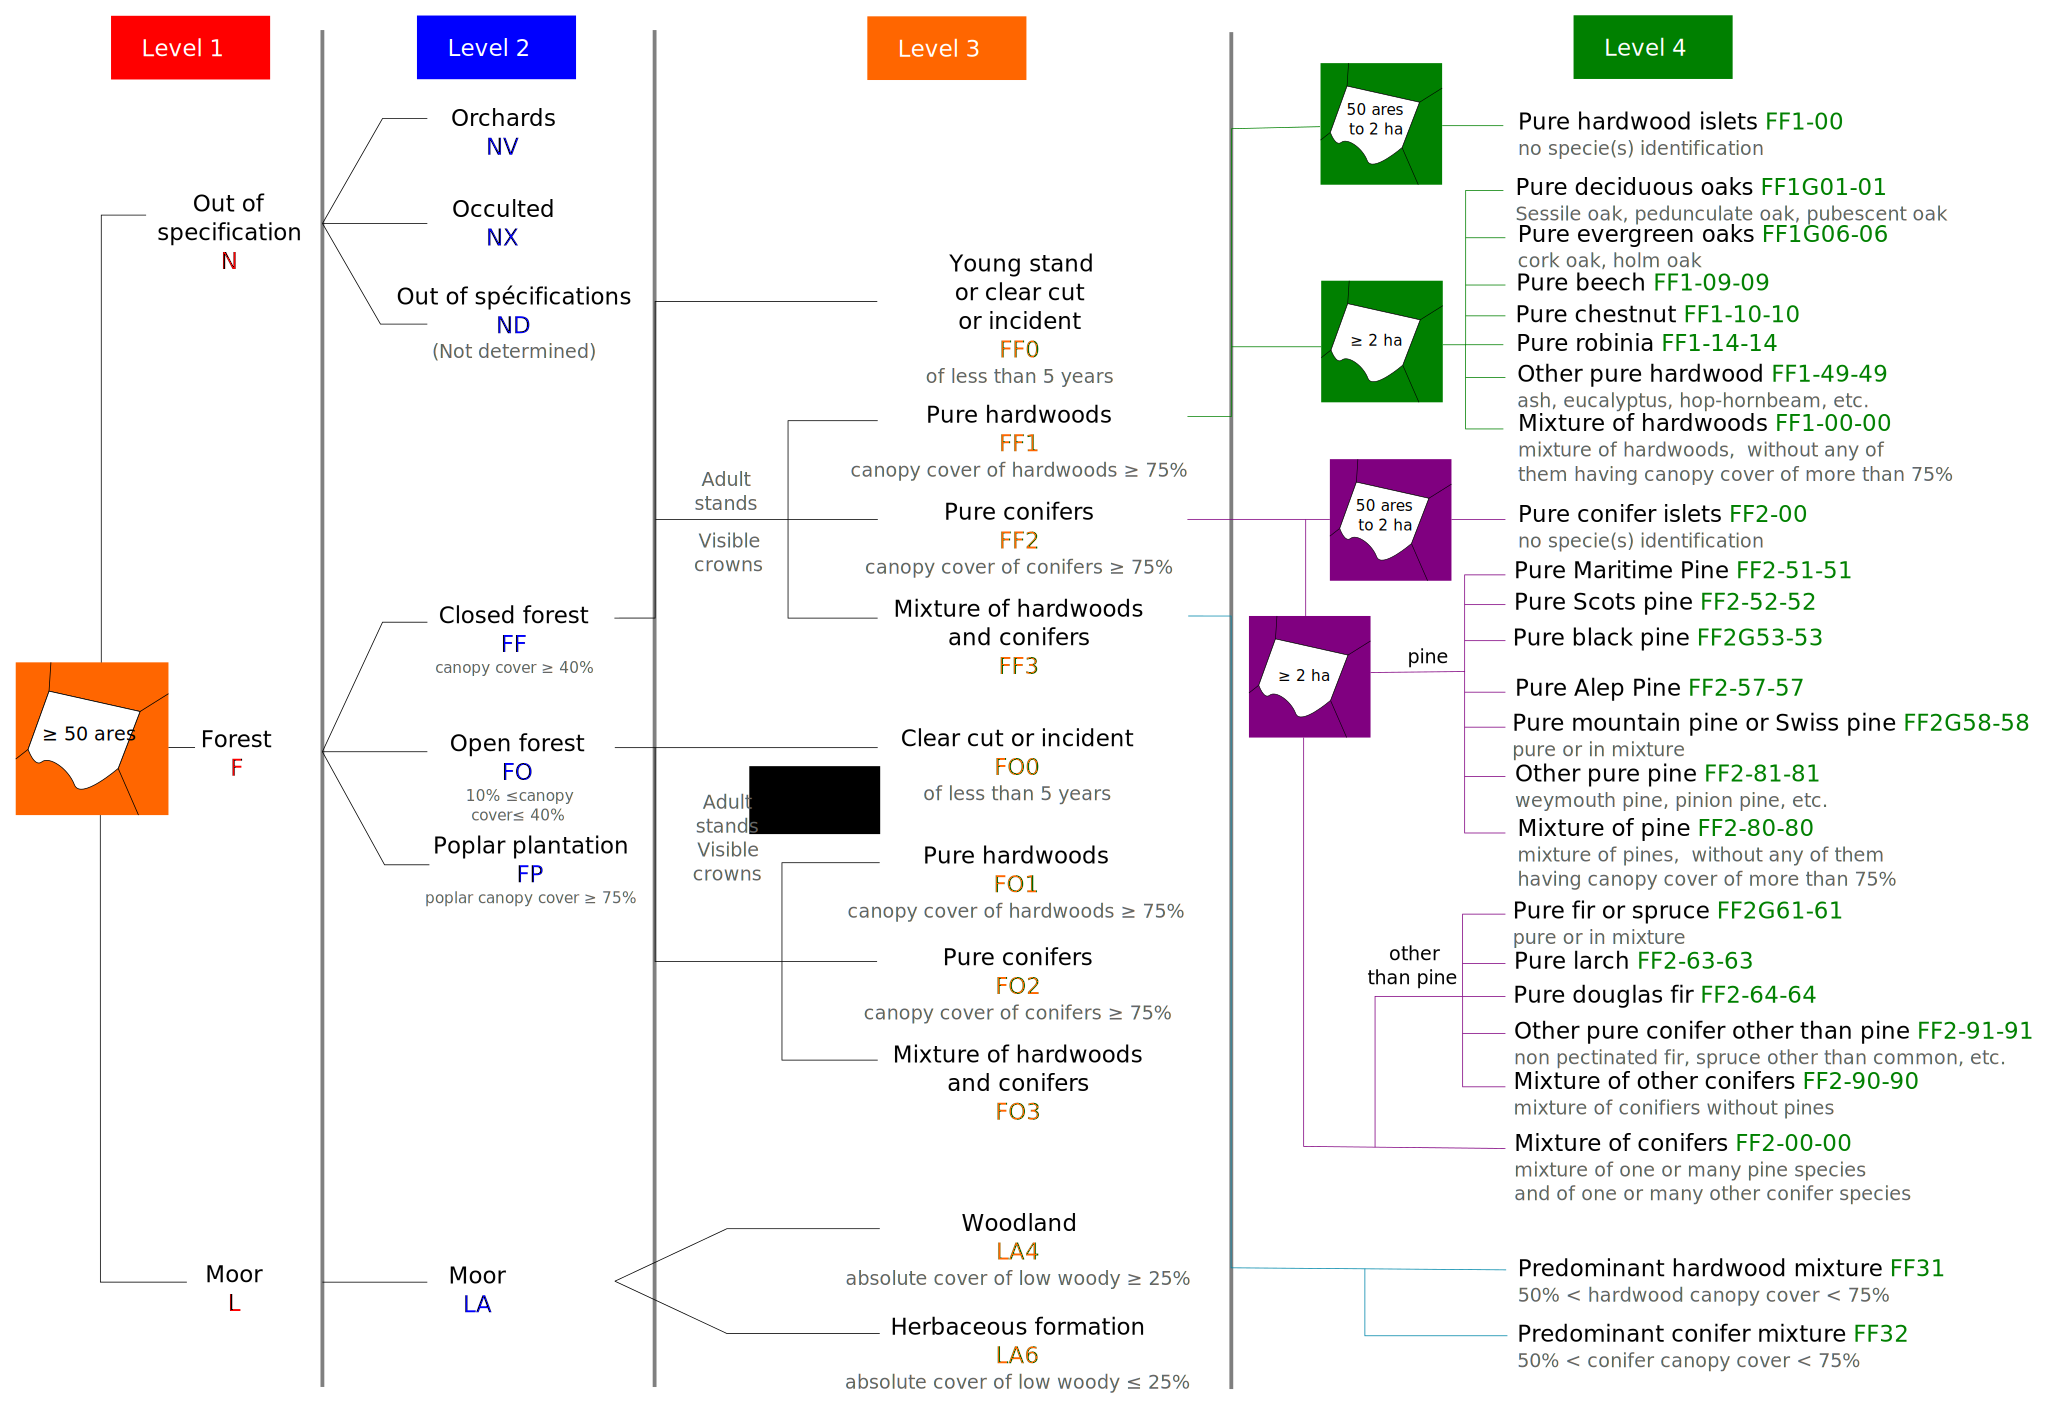
\includegraphics[width=\textwidth]{Figures/v2_organigram}
\caption{Organizational chart of the version 2 of the forest LC database.}
\label{fig:organigram_BD}
\end{center}
\end{figure}


\section{Segmentation methods}
A naive method to retrieve forest stands is to segment the input data. Such segmentation algorithms do not take into account the species information. Two algorithms were employed in order to obtain relevant stands only through the segmentation of the data.
The first segmentation algorithm is the one proposed in \cite{guigues2006scale}. It is a hierarchical segmentation algorithm that allows to control the level of segmentation through a unique scale parameter $\mu$.

The second segmentation algorithm (called PFF) employed is presented in \cite{felzenszwalb2004efficient}. It is a method for image segmentation based on pairwise region comparison considering the minimum weight edge between two regions in measuring the difference between them. 3 simples parameters need to be tuned in order to obtain relevant segmentation. $\sigma$ is the standard deviation of the gaussian filter employed to smooth the image as a pre-processing (the authors recommend $\sigma=0.8$). $k$ is a second parameter that set a scale of observation (a larger $k$ will lead to larger segments). Finally, the parameter $m$ permits to define the minimum size of a segment.

Such segmentation could allow to retrieve the stands borders easily. Furthermore, one the segmentation is performed, one can add semantic information using classification results.

These experiments have been performed only on one area presented in Figure~\ref{fig:data_direct_seg}. It is a 1$\:$km$^{2}$ area, the spatial resolution of the VHR optical image is 0.5$\:$m, and the nDSM has been rasterized at the same resolution. From these data one can see that a stand is composed of zones that are not homogeneous in term of reflectance and/or height. Furthermore, one can also note that the variability between two stands in terms of reflectance and/or height might not be important.

\begin{figure}[htbp]
\begin{center}
\begingroup
\captionsetup[subfigure]{width=0.16\textwidth}
\subfloat[VHR IRC optical image.]{
\includegraphics[width=0.3\textwidth]{Figures/C3/S2/IRC}
\label{subfig:hierar3}
}
\subfloat[nDSM.]{
\includegraphics[width=0.3\textwidth]{Figures/C3/S2/nDSM}
\label{subfig:hierar3}
}
\subfloat[Forest LC database.]{
\includegraphics[width=0.3\textwidth]{Figures/C3/S2/BD}
\label{subfig:hierar3}
}
\endgroup
\caption{VHR IRC optical image, rasterized nDSM and forest LC of the proposed area for the direct segmentation tests.}
\label{fig:data_direct_seg}
\end{center}
\end{figure}

\subsection{Retrieve stands borders}

Two strategies are employed to apply the segmentation in order to retrieve the forest stands borders from the forest LC database:
\begin{itemize}
\item The segmentation is applied to the VHR optical images, thus the resulting segment will correspond to "stands" that are homogeneous in terms of spectral reflectance. Since the optical images are employed by photo-interpreters in order to derive the forest LC, such segmentation should produce results similar to the forest LC.
\item The segmentation is also applied to the rasterized normalized digital surface model (nDSM) (canopy height without ground relief). Such segmentation would produce "stands" that are homogeneous in term of height.
\end{itemize}

The results of the segmentation of the VHR optical image using the two segmentation algorithm is presented in Figure~\ref{fig:seg_im}. In both cases, most of the borders found are not consistent with the forest LC database. Visually, the hierarchical segmentation seems to be more relevant than the PFF segmentation. However, the hierarchical segmentation produces small segments due to high variation of illumination in the image, while the PFF segments are all relatively large. 

\begin{figure}[htbp]
\begin{center}
\begingroup
\captionsetup[subfigure]{width=0.4\textwidth}
\subfloat[Hierarchical segmentation with $\mu=15$.]{
\includegraphics[width=0.45\textwidth]{Figures/C3/S2/border_hierar}
\label{subfig:hierar3}
}
\hspace*{0.05\textwidth}
\subfloat[PFF segmentation with $\sigma=0.8$, $k=500$ and $m=40000$.]{
\includegraphics[width=0.45\textwidth]{Figures/C3/S2/border_PFF_IRC}
\label{subfig:hierar3}
}
\endgroup
\caption{Result of the segmentation of the VHR optical image for the two segmentation algorithms. Blue lines correspond to the borders of the segments, red lines correspond to the borders of the forest LC.}
\label{fig:seg_im}
\end{center}
\end{figure}

The results of the segmentation of rasterized nDSM using the two segmentation algorithm is presented in Figure~\ref{fig:seg_nDSM}. Just like the segmentation of the VHR optical image, most of the borders found are not consistent with the forest LC database. Here, the PFF segmentation seems to perform better than the hierarchical segmentation visually.


\begin{figure}[htbp]
\begin{center}
\begingroup
\captionsetup[subfigure]{width=0.4\textwidth}
\subfloat[Hierarchical segmentation with $\mu=15$.]{
\includegraphics[width=0.45\textwidth]{Figures/C3/S2/border_hierar_z}
\label{subfig:hierar3}
}
\hspace*{0.05\textwidth}
\subfloat[PFF segmentation with $\sigma=0.8$, $k=500$ and $m=40000$.]{
\includegraphics[width=0.45\textwidth]{Figures/C3/S2/border_PFF_z}
\label{subfig:hierar3}
}
\endgroup
\caption{Result of the segmentation of the nDSM for the two segmentation algorithms. Blue lines correspond to the borders of the segments, red lines correspond to the borders of the forest LC.}
\label{fig:seg_nDSM}
\end{center}
\end{figure}

Since the segmentation on the VHR optical image and the nDSM does not allow to retrieve the borders from the forest LC database, different values of the parameter $\mu$ for the hierarchical segmentation on the VHR optical images (see Figure~\ref{fig:hierar}). It appears that decreasing $\mu$ does not allow to obtain the borders of the forest LC. It only leads to and over-segmentation of the image. Such over-segmentation is employed in the proposed method but is not employed as a relevant segmentation for stand delineation but as an input for object based classification.

\begin{figure}[htbp]
\begin{center}
\begingroup
\captionsetup[subfigure]{width=0.5\textwidth}
\subfloat[Hierarchical segmentation with $\mu=3$.]{
\includegraphics[width=0.45\textwidth]{Figures/C3/S2/seg_herarchical_3border_hierarchical}
\label{subfig:hierar3}
}
\hspace*{0.05\textwidth}
\subfloat[Hierarchical segmentation with $\mu=6$.]{
\includegraphics[width=0.45\textwidth]{Figures/C3/S2/seg_herarchical_6border_hierarchical}
\label{subfig:hierar6}
}
\\
\subfloat[Hierarchical segmentation with $\mu=8$.]{
\includegraphics[width=0.45\textwidth]{Figures/C3/S2/seg_herarchical_8border_hierarchical}
\label{subfig:hierar8}
}
\hspace*{0.05\textwidth}
\subfloat[Hierarchical segmentation with $\mu=10$.]{
\includegraphics[width=0.45\textwidth]{Figures/C3/S2/seg_herarchical_10border_hierarchical}
\label{subfig:hierar10}
}
\\
\subfloat[Hierarchical segmentation with $\mu=12$.]{
\includegraphics[width=0.45\textwidth]{Figures/C3/S2/seg_herarchical_12border_hierarchical}
\label{subfig:hierar12}
}
\hspace*{0.05\textwidth}
\subfloat[Hierarchical segmentation with $\mu=15$.]{
\includegraphics[width=0.45\textwidth]{Figures/C3/S2/seg_herarchical_15border_hierarchical}
\label{subfig:hierar15}
}
\endgroup
\caption{Result of the segmentation of the VHR optical image using different values of $\mu$ for the hierarchical segmentation. Blue lines correspond to the borders of the segments, red lines correspond to the borders of the forest LC.}
\label{fig:hierar}
\end{center}
\end{figure}

The two proposed segmentation algorithms are very efficient for image segmentation tasks \citep{guigues2006scale, felzenszwalb2004efficient} but are not adapted to retrieve forest stands borders. However, they can produce interesting over-segmentation since they are able to retrieve some relevant borders.

\subsection{Add semantic information}
The classification proposed in the method give information about the species at the object level. Since the segments extracted below are large than the small objects, a majority vote can be applied for each segment. The obtained label map could be compared with the forest LC.
The result of the classification for the area of interest is presented in Figure~\ref{fig:C3_S2_classif}, the confusion matrix and other accuracy metrics for this classification are presented in Table~\ref{table:C
_S2_classif}.

\begin{figure}[htbp]
\begin{center}
\begingroup
\captionsetup[subfigure]{width=0.375\textwidth}
\subfloat[Forest LC.]{
\includegraphics[width=0.45\textwidth]{Figures/C3/S2/BD}
\label{subfig:hierar3}
}
\hspace*{0.05\textwidth}
\subfloat[Classification results (overall accuracy: 81.75\%, $\kappa$:0.67).]{
\includegraphics[width=0.45\textwidth]{Figures/C3/S2/classif}
\label{subfig:hierar3}
}
\endgroup
\caption{Forest LC and classification results.}
\label{fig:C3_S2_classif}
\end{center}
\end{figure}



\section{Results of the method}
\subsection{Over-segmentation}
\subsection{Feature selection}
\subsection{Classification}
\subsection{Regularization}
\section{Co-products of the method}
\section{Semi-automatic update}
\section{Inventory}
%----------------------------------------------------------------------------------------

% Define some commands to keep the formatting separated from the content 
%\newcommand{\keyword}[1]{\textbf{#1}}
%\newcommand{\tabhead}[1]{\textbf{#1}}
%\newcommand{\code}[1]{\texttt{#1}}
%\newcommand{\file}[1]{\texttt{\bfseries#1}}
%\newcommand{\option}[1]{\texttt{\itshape#1}}

%----------------------------------------------------------------------------------------


\stopcontents[chapters]